\documentclass[10pt]{extarticle}
\usepackage[letterpaper, margin=1in]{geometry}
\usepackage{amsmath}
\usepackage{amssymb}
\usepackage{enumitem}
\usepackage{fancyhdr}
\usepackage{graphicx}
\usepackage{lastpage}
\usepackage{tcolorbox}

\allowdisplaybreaks
\setlength{\parindent}{0pt}

\title{\centering\Large\textsc{Applications of Linear Algebra: Problem Set 4}}
\author{\large \textsc{Rento Saijo}}
\date{May 12, 2026}

\pagestyle{fancy}
\fancyhf{}
\fancyfoot[C]{\textsc{Page \thepage\ of \pageref{LastPage}}}
\renewcommand{\headrulewidth}{0pt}

\newtcolorbox{problem}[1][]{
    colframe=darkgray!100,
    arc=0.1mm,
    boxrule=2pt,
    boxsep=1mm,
    title={\textsc{#1}}
}

\begin{document}
\maketitle
\thispagestyle{fancy}
\vspace{-1em}\noindent\rule{\linewidth}{0.6pt}\vspace{0.5em}

\begin{problem}[Problem 1]
A student runs an experiment six times in an attempt to obtain an equation relating two physical quantities $x$ and $y$. For $x=1,2,4,6,8,10$ units, the experiments result in corresponding $y$ values of $3,3,4,6,7,8$.
\begin{enumerate}[label=(\alph*)]
\item Find and compare the graphs of the following:
\begin{enumerate}[label=(\roman*)]
\item the least squares line;
\item the least squares quadratic polynomial; and
\item the interpolating polynomial.
\end{enumerate}
\item Which do you think is the most likely theoretical model for this data? Why?
\end{enumerate}
\end{problem}

\begin{enumerate}[label=(\alph*)]
\item We start with the least squares line $y=mx+b$. If
\[
A=
\begin{pmatrix}
1 & 1\\
2 & 1\\
4 & 1\\
6 & 1\\
8 & 1\\
10 & 1
\end{pmatrix},
\qquad
\vec{y}=
\begin{pmatrix}
3\\3\\4\\6\\7\\8
\end{pmatrix},
\]
then the normal equations are
\[
A^TA
\begin{pmatrix}
m\\b
\end{pmatrix}
=
A^T\vec{y}.
\]
Here,
\[
A^TA=
\begin{pmatrix}
221 & 31\\
31 & 6
\end{pmatrix},
\qquad
A^T\vec{y}=
\begin{pmatrix}
197\\
31
\end{pmatrix}.
\]
So we solve
\[
\begin{pmatrix}
221 & 31\\
31 & 6
\end{pmatrix}
\begin{pmatrix}
m\\b
\end{pmatrix}
=
\begin{pmatrix}
197\\
31
\end{pmatrix},
\]
which gives
\[
m=\frac{221}{365},
\qquad
b=\frac{744}{365}.
\]
Therefore, the least squares line is
\[
y=\frac{221}{365}x+\frac{744}{365}.
\]

Now, do the same thing for a quadratic model
\[
y=ax^2+bx+c.
\]
This time,
\[
A=
\begin{pmatrix}
1 & 1 & 1\\
4 & 2 & 1\\
16 & 4 & 1\\
36 & 6 & 1\\
64 & 8 & 1\\
100 & 10 & 1
\end{pmatrix},
\qquad
\vec{y}=
\begin{pmatrix}
3\\3\\4\\6\\7\\8
\end{pmatrix},
\]
so the normal equations become
\[
A^TA
\begin{pmatrix}
a\\b\\c
\end{pmatrix}
=
A^T\vec{y}.
\]
We compute
\[
A^TA=
\begin{pmatrix}
15665 & 1801 & 221\\
1801 & 221 & 31\\
221 & 31 & 6
\end{pmatrix},
\qquad
A^T\vec{y}=
\begin{pmatrix}
1543\\
197\\
31
\end{pmatrix}.
\]
Solving this system gives
\[
a=\frac{25}{4652},
\qquad
b=\frac{12729}{23260},
\qquad
c=\frac{24903}{11630}.
\]
So the least squares quadratic is
\[
y=\frac{25}{4652}x^2+\frac{12729}{23260}x+\frac{24903}{11630}.
\]

For the interpolating polynomial, the $x$-values are all distinct, so the Vandermonde matrix is regular. Therefore, there is a unique interpolating polynomial of degree at most $5$. Write
\[
p(x)=c_5x^5+c_4x^4+c_3x^3+c_2x^2+c_1x+c_0.
\]
Then, the coefficients satisfy
\[
\begin{pmatrix}
1^5 & 1^4 & 1^3 & 1^2 & 1 & 1\\
2^5 & 2^4 & 2^3 & 2^2 & 2 & 1\\
4^5 & 4^4 & 4^3 & 4^2 & 4 & 1\\
6^5 & 6^4 & 6^3 & 6^2 & 6 & 1\\
8^5 & 8^4 & 8^3 & 8^2 & 8 & 1\\
10^5 & 10^4 & 10^3 & 10^2 & 10 & 1
\end{pmatrix}
\begin{pmatrix}
c_5\\c_4\\c_3\\c_2\\c_1\\c_0
\end{pmatrix}
=
\begin{pmatrix}
3\\3\\4\\6\\7\\8
\end{pmatrix}.
\]
Solving this system gives
\[
p(x)=
\frac{169}{120960}x^5
-\frac{275}{8064}x^4
+\frac{419}{1512}x^3
-\frac{535}{672}x^2
+\frac{6931}{7560}x
+\frac{166}{63}.
\]

On the graph below (via Python), the least squares line and the least squares quadratic are very close to each other. The quadratic does bend upward a little bit, but the bend is small because the coefficient of $x^2$ is only
\[
\frac{25}{4652}\approx 0.005374.
\]
The interpolating polynomial is the one that passes through every single data point exactly, but it also has the most freedom to wiggle between the data points.

\[
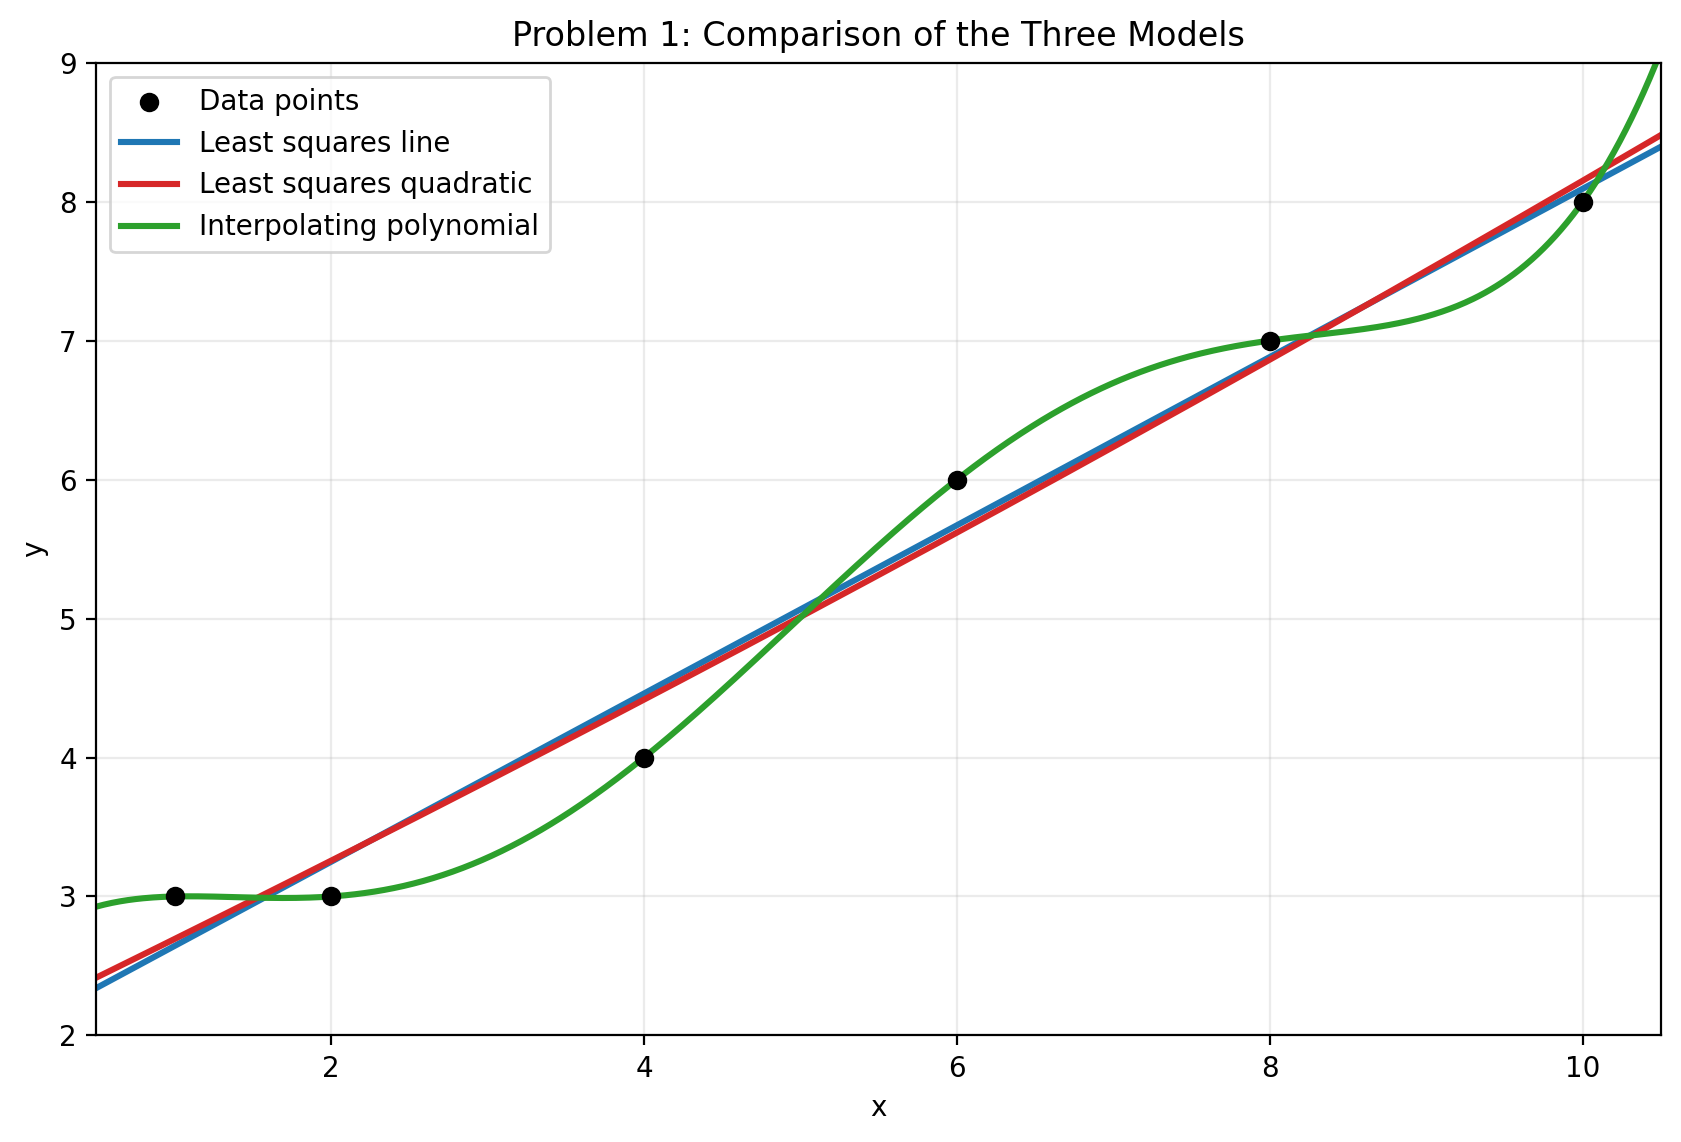
\includegraphics[width=0.9\textwidth]{homework4_problem1_graph.png}
\]

\item The least squares line seems like the most likely theoretical model. The main reason is that the data has a pretty clear overall linear upward trend, and the quadratic fit only improves the least squares error by a very small amount. For the line, the fitted values at the six data points are
\[
\frac{193}{73},\qquad
\frac{1186}{365},\qquad
\frac{1628}{365},\qquad
\frac{414}{73},\qquad
\frac{2512}{365},\qquad
\frac{2954}{365}.
\]
So the residuals are
\[
3-\frac{193}{73}=\frac{26}{73},\qquad
3-\frac{1186}{365}=-\frac{91}{365},\qquad
4-\frac{1628}{365}=-\frac{168}{365},
\]
\[
6-\frac{414}{73}=\frac{24}{73},\qquad
7-\frac{2512}{365}=\frac{43}{365},\qquad
8-\frac{2954}{365}=-\frac{34}{365}.
\]
Therefore,
\[
\text{SSE for the line}
=\left(\frac{26}{73}\right)^2
+\left(-\frac{91}{365}\right)^2
+\left(-\frac{168}{365}\right)^2
+\left(\frac{24}{73}\right)^2
+\left(\frac{43}{365}\right)^2
+\left(-\frac{34}{365}\right)^2
=\frac{194}{365}\approx 0.5315,
\]
while for the quadratic, the fitted values are
\[
\frac{3133}{1163},\qquad
\frac{18941}{5815},\qquad
\frac{51361}{11630},\qquad
\frac{6534}{1163},\qquad
\frac{79819}{11630},\qquad
\frac{47399}{5815}.
\]
So the residuals are
\[
3-\frac{3133}{1163}=\frac{356}{1163},\qquad
3-\frac{18941}{5815}=-\frac{1496}{5815},\qquad
4-\frac{51361}{11630}=-\frac{4841}{11630},
\]
\[
6-\frac{6534}{1163}=\frac{444}{1163},\qquad
7-\frac{79819}{11630}=\frac{1591}{11630},\qquad
8-\frac{47399}{5815}=-\frac{879}{5815}.
\]
Therefore,
\[
\begin{aligned}
\text{SSE for the quadratic}
&=\left(\frac{356}{1163}\right)^2
+\left(-\frac{1496}{5815}\right)^2
+\left(-\frac{4841}{11630}\right)^2\\
&\quad
+\left(\frac{444}{1163}\right)^2
+\left(\frac{1591}{11630}\right)^2
+\left(-\frac{879}{5815}\right)^2\\
&=\frac{6053}{11630}\approx 0.5205.
\end{aligned}
\]
So the quadratic is technically a better least squares fit, but not by enough to strongly suggest that the true model should be quadratic. The interpolating polynomial is the one I would trust the least as a theoretical model, because it is built to hit every data point exactly, including any experimental noise. So, the ranking is
\[
\text{line first, quadratic second, interpolating polynomial last.}
\]
Essentially, the latter 2 models are overfitting to the training data and won't be stable for test data if this training trend is representative of the test trend.
\end{enumerate}

\newpage

\begin{problem}[Problem 2]
Let $q(t)$ denote the quadratic interpolating polynomial that goes through the data points $(t_0,y_0),(t_1,y_1),(t_2,y_2)$.
\begin{enumerate}[label=(\alph*)]
\item Find and simplify the coefficients $a,b,c$ of $q(t)=at^2-bt+c$.
\item What must be true for $q(t)$ to have a minimum? A maximum?
\item Show that the minimizing/maximizing value of $q(t)$ is at
\[
t^*=\frac{m_0s_1-m_1s_0}{s_1-s_0}
\]
where
\[
s_0=\frac{y_1-y_0}{t_1-t_0},
\qquad
s_1=\frac{y_2-y_1}{t_2-t_1},
\qquad
m_0=\frac{t_0+t_1}{2},
\qquad
m_1=\frac{t_1+t_2}{2}.
\]
\item Give the minimum/maximum value $q(t^*)$.
\end{enumerate}
\end{problem}

\begin{enumerate}[label=(\alph*)]
\item Since the interpolating polynomial is
\[
q(t)=at^2-bt+c,
\]
and it passes through $(t_0,y_0),(t_1,y_1),(t_2,y_2)$, the coefficients satisfy the linear system
\[
\begin{pmatrix}
t_0^2 & -t_0 & 1\\
t_1^2 & -t_1 & 1\\
t_2^2 & -t_2 & 1
\end{pmatrix}
\begin{pmatrix}
a\\b\\c
\end{pmatrix}
=
\begin{pmatrix}
y_0\\y_1\\y_2
\end{pmatrix}.
\]
Equivalently, the augmented matrix is
\[
\left(
\begin{array}{ccc|c}
t_0^2 & -t_0 & 1 & y_0\\
t_1^2 & -t_1 & 1 & y_1\\
t_2^2 & -t_2 & 1 & y_2
\end{array}
\right).
\]
Now, subtract the first row from the second, and subtract the second row from the third:
\[
R_2\leftarrow R_2-R_1,
\qquad
R_3\leftarrow R_3-R_2.
\]
This gives
\[
\left(
\begin{array}{ccc|c}
t_0^2 & -t_0 & 1 & y_0\\
t_1^2-t_0^2 & -(t_1-t_0) & 0 & y_1-y_0\\
t_2^2-t_1^2 & -(t_2-t_1) & 0 & y_2-y_1
\end{array}
\right).
\]
Since
\[
t_1^2-t_0^2=(t_1-t_0)(t_1+t_0),
\qquad
t_2^2-t_1^2=(t_2-t_1)(t_2+t_1),
\]
we can divide the second row by $t_1-t_0$ and the third row by $t_2-t_1$:
\[
R_2\leftarrow \frac{1}{t_1-t_0}R_2,
\qquad
R_3\leftarrow \frac{1}{t_2-t_1}R_3.
\]
Then,
\[
\left(
\begin{array}{ccc|c}
t_0^2 & -t_0 & 1 & y_0\\
t_1+t_0 & -1 & 0 & \dfrac{y_1-y_0}{t_1-t_0}\\[0.9em]
t_2+t_1 & -1 & 0 & \dfrac{y_2-y_1}{t_2-t_1}
\end{array}
\right).
\]
To keep the notation shorter, I should let
\[
s_0=\frac{y_1-y_0}{t_1-t_0},
\qquad
s_1=\frac{y_2-y_1}{t_2-t_1}.
\]
So the augmented matrix becomes
\[
\left(
\begin{array}{ccc|c}
t_0^2 & -t_0 & 1 & y_0\\
t_1+t_0 & -1 & 0 & s_0\\[0.4em]
t_2+t_1 & -1 & 0 & s_1
\end{array}
\right).
\]
Now, subtract the second row from the third:
\[
R_3\leftarrow R_3-R_2.
\]
Then,
\[
\left(
\begin{array}{ccc|c}
t_0^2 & -t_0 & 1 & y_0\\
t_1+t_0 & -1 & 0 & s_0\\[0.4em]
t_2-t_0 & 0 & 0 & s_1-s_0
\end{array}
\right).
\]
Now, divide the third row by $t_2-t_0$:
\[
R_3\leftarrow \frac{1}{t_2-t_0}R_3.
\]
This gives
\[
\left(
\begin{array}{ccc|c}
t_0^2 & -t_0 & 1 & y_0\\
t_1+t_0 & -1 & 0 & s_0\\[0.4em]
1 & 0 & 0 & \dfrac{s_1-s_0}{t_2-t_0}
\end{array}
\right).
\]
So we can already read off
\[
a=\frac{s_1-s_0}{t_2-t_0}.
\]
Next, eliminate the $a$-entry from the second row:
\[
R_2\leftarrow R_2-(t_1+t_0)R_3.
\]
Then,
\[
\left(
\begin{array}{ccc|c}
t_0^2 & -t_0 & 1 & y_0\\
0 & -1 & 0 & s_0-(t_1+t_0)a\\[0.4em]
1 & 0 & 0 & a
\end{array}
\right).
\]
Finally, multiply the second row by $-1$:
\[
R_2\leftarrow -R_2,
\]
so
\[
\left(
\begin{array}{ccc|c}
t_0^2 & -t_0 & 1 & y_0\\
0 & 1 & 0 & (t_1+t_0)a-s_0\\[0.4em]
1 & 0 & 0 & a
\end{array}
\right).
\]
Thus,
\[
b=(t_1+t_0)a-s_0.
\]
If we let
\[
m_0=\frac{t_0+t_1}{2},
\qquad
m_1=\frac{t_1+t_2}{2},
\]
then this is the same as
\[
b=2am_0-s_0=2am_1-s_1.
\]
To get $c$, eliminate the $a$ and $b$ entries from the first row:
\[
R_1\leftarrow R_1-t_0^2R_3,
\qquad
R_1\leftarrow R_1+t_0R_2.
\]
This gives
\[
\left(
\begin{array}{ccc|c}
0 & 0 & 1 & y_0-t_0^2a+t_0b\\
0 & 1 & 0 & b\\
1 & 0 & 0 & a
\end{array}
\right),
\]
so
\[
c=y_0-t_0^2a+t_0b.
\]
Therefore, the coefficients are
\[
a=\frac{s_1-s_0}{t_2-t_0},
\qquad
b=2am_0-s_0,
\qquad
c=y_0-at_0^2+bt_0.
\]

\item From part (a), we already know
\[
a=\frac{s_1-s_0}{t_2-t_0}.
\]
Since
\[
q(t)=at^2-bt+c,
\]
its derivative is
\[
q'(t)=2at-b.
\]
So the graph is an upward-opening parabola if $a>0$ and a downward-opening parabola if $a<0$. That means:
\[
\text{minimum if } a>0,
\qquad
\text{maximum if } a<0.
\]
So, in terms of the quantities from part (a),
\[
\text{minimum if } \frac{s_1-s_0}{t_2-t_0}>0,
\qquad
\text{maximum if } \frac{s_1-s_0}{t_2-t_0}<0.
\]
If $a=0$, then the polynomial is not really quadratic anymore, so there is no genuine parabolic minimum or maximum to talk about.

\item The critical point happens when
\[
q'(t)=2at-b=0,
\]
so
\[
t^*=\frac{b}{2a}.
\]
Now, use the coefficient relation from part (a),
\[
b=2am_0-s_0=2am_1-s_1.
\]
Rearranging gives
\[
s_0=2am_0-b,
\qquad
s_1=2am_1-b.
\]
Subtract these:
\[
s_1-s_0=2a(m_1-m_0).
\]
Also,
\[
m_0s_1-m_1s_0
=m_0(2am_1-b)-m_1(2am_0-b).
\]
The $2am_0m_1$ terms cancel, so this becomes
\[
m_0s_1-m_1s_0=b(m_1-m_0).
\]
Therefore,
\[
\frac{m_0s_1-m_1s_0}{s_1-s_0}
=\frac{b(m_1-m_0)}{2a(m_1-m_0)}
=\frac{b}{2a}
=t^*.
\]
So indeed,
\[
t^*=\frac{m_0s_1-m_1s_0}{s_1-s_0}.
\]

\item Using the same coefficients from part (a), complete the square:
\[
q(t)=at^2-bt+c
=a\left(t-\frac{b}{2a}\right)^2+c-\frac{b^2}{4a}.
\]
Since
\[
t^*=\frac{b}{2a},
\]
we get
\[
q(t^*)=c-\frac{b^2}{4a}.
\]
So the minimum or maximum value is
\[
\boxed{q(t^*)=c-\frac{b^2}{4a}}.
\]
If $a>0$, this is the minimum value. If $a<0$, this is the maximum value.
\end{enumerate}

\newpage

\begin{problem}[Problem 3]
This problem sits in the context of approximating data points $(t_1,y_1),(t_2,y_2),\dots,(t_m,y_m)$ with polynomials. To find the coefficients of the least squares approximating polynomial, we developed an orthogonal basis $q_0(t),q_1(t),q_2(t),\dots$ and used that to get an orthogonal set of sampling points of the data $\mathbf{q}_0,\mathbf{q}_1,\mathbf{q}_2,\dots$:
\[
\setlength\arraycolsep{15pt}
\begin{array}{lll}
q_0(t)=1, & \mathbf{q}_0=\mathbf{t}_0, & \lVert \mathbf{q}_0\rVert^2=1,\\
q_1(t)=t, & \mathbf{q}_1=\mathbf{t}_1, & \lVert \mathbf{q}_1\rVert^2=\overline{t^2},\\
q_2(t)=t^2-\overline{t^2}, & \mathbf{q}_2=\mathbf{t}_2-\overline{t^2}\mathbf{t}_0, & \lVert \mathbf{q}_2\rVert^2=\overline{t^4}-\left(\overline{t^2}\right)^2,\\
q_3(t)=t^3-\dfrac{\overline{t^4}}{\overline{t^2}}t, & \mathbf{q}_3=\mathbf{t}_3-\dfrac{\overline{t^4}}{\overline{t^2}}\mathbf{t}_1, & \lVert \mathbf{q}_3\rVert^2=\overline{t^6}-\dfrac{\left(\overline{t^4}\right)^2}{\overline{t^2}},
\end{array}
\]
where
\[
\mathbf{t}_k=\begin{pmatrix}t_1^k,t_2^k,\dots,t_m^k\end{pmatrix}^T
\qquad \text{and} \qquad
\overline{t^k}=\frac{1}{m}\sum_{i=1}^m t_i^k.
\]
When we generated these polynomials, we made some simplifying assumptions, namely that the $t$-coordinates of the data points are uniformly distributed about $t=0$. As long as the data is uniformly distributed, we can convert the least squares problem to the symmetric form as follows.
\begin{enumerate}[label=(\alph*)]
\item Assume $t_{i+1}-t_i=h$ for all $i=1,\dots,m-1$. Show that the translated sample points $s_i=t_i-\overline{t}$, where
\[
\overline{t}=\frac{1}{m}\sum_{i=1}^m t_i,
\]
are symmetric around $0$.
\item Suppose that $q(s)$ is the least squares polynomial for the data points $(s_i,y_i)$. Show that $p(t)=q(1-t)$ is the least squares polynomial for the original data $(t_i,y_i)$.
\item Apply this method to find the least squares polynomials of degrees $1$, $2$, and $3$ for the following data:
\[
\begin{array}{c|cccccc}
t_i & 1 & 2 & 3 & 4 & 5 & 6 \\ \hline
y_i & -8 & -6 & -4 & -1 & 1 & 3
\end{array}.
\]
\end{enumerate}
\end{problem}

\begin{enumerate}[label=(\alph*)]
\item Since the $t_i$ are equally spaced, each new point is obtained by adding the same step size $h$. So
\[
t_i=t_1+(i-1)h.
\]
The last point is
\[
t_m=t_1+(m-1)h,
\]
so the midpoint of the first and last points is
\[
\frac{t_1+t_m}{2}
=\frac{t_1+t_1+(m-1)h}{2}
=t_1+\frac{m-1}{2}h.
\]
For equally spaced points, this midpoint is also the average value, so
\[
\overline{t}=t_1+\frac{m-1}{2}h.
\]
Therefore,
\[
s_i=t_i-\overline{t}
=t_1+(i-1)h-\left(t_1+\frac{m-1}{2}h\right)
=\left(i-\frac{m+1}{2}\right)h.
\]
Now, check the point paired with $s_i$, namely $s_{m+1-i}$:
\[
s_{m+1-i}
=\left((m+1-i)-\frac{m+1}{2}\right)h
=\left(\frac{m+1}{2}-i\right)h
=-s_i.
\]
So the translated points come in opposite pairs, which is exactly what it means to be symmetric around $0$.

\item From part (a), the shifted variable is
\[
s=t-\overline{t},
\]
so the corresponding polynomial for the original variable should be
\[
p(t)=q(t-\overline{t}).
\]
The shift coming from part (a) depends on $\overline{t}$, not on the fixed number $1$, it seems. Also, to recover the original data, we need
\[
p(t_i)=q(s_i)=q(t_i-\overline{t})
\]
at every sample point. But $q(1-t_i)$ would usually give different inputs, so it would not match the shifted least squares problem unless we happened to be in a very special case. So I'm going to assume that it was supposed to be
\[
p(t)=q(t-\overline{t}).
\]
Now, let $p(t)$ be any polynomial of the same degree, and define
\[
r(s)=p(s+\overline{t}).
\]
Then, at the sample points, since $s_i=t_i-\overline{t}$, we have
\[
r(s_i)=p(t_i).
\]
So the least squares error for the original data is
\[
\sum_{i=1}^m \left(y_i-p(t_i)\right)^2
=\sum_{i=1}^m \left(y_i-r(s_i)\right)^2.
\]
But $q(s)$ is assumed to be the least squares polynomial for the shifted data $(s_i,y_i)$, so
\[
\sum_{i=1}^m \left(y_i-q(s_i)\right)^2
\le
\sum_{i=1}^m \left(y_i-r(s_i)\right)^2.
\]
Replace $r(s_i)$ by $p(t_i)$:
\[
\sum_{i=1}^m \left(y_i-q(s_i)\right)^2
\le
\sum_{i=1}^m \left(y_i-p(t_i)\right)^2.
\]
Now, define
\[
p(t)=q(t-\overline{t}).
\]
Then
\[
p(t_i)=q(s_i),
\]
so $p(t)$ is the least squares polynomial for the original data.

\item For this data,
\[
t_1=1,\qquad t_2=2,\qquad t_3=3,\qquad t_4=4,\qquad t_5=5,\qquad t_6=6.
\]
Their average is
\[
\overline{t}=\frac{1+2+3+4+5+6}{6}=\frac{7}{2}.
\]
So the translated points are
\[
s_i=t_i-\frac{7}{2},
\]
namely
\[
-\frac{5}{2},\quad -\frac{3}{2},\quad -\frac{1}{2},\quad \frac{1}{2},\quad \frac{3}{2},\quad \frac{5}{2}.
\]
These are symmetric around $0$, just as we derived in part (a), so it makes sense to shift; once the sample points are centered around $0$, we can use the orthogonal basis formulas from the problem statement directly. Then, after finding the least squares polynomial in the shifted variable $s$, part (b) tells us how to return to the original variable $t$, namely by substituting
\[
s=t-\frac{7}{2}.
\]
Let
\[
\mathbf{s}_0=
\begin{pmatrix}
1\\1\\1\\1\\1\\1
\end{pmatrix},
\qquad
\mathbf{s}_1=
\begin{pmatrix}
-\frac{5}{2}\\[0.3em]
-\frac{3}{2}\\[0.3em]
-\frac{1}{2}\\[0.3em]
\frac{1}{2}\\[0.3em]
\frac{3}{2}\\[0.3em]
\frac{5}{2}
\end{pmatrix}.
\]
The next sample vectors are
\[
\mathbf{s}_2=
\begin{pmatrix}
\frac{25}{4}\\[0.3em]
\frac{9}{4}\\[0.3em]
\frac{1}{4}\\[0.3em]
\frac{1}{4}\\[0.3em]
\frac{9}{4}\\[0.3em]
\frac{25}{4}
\end{pmatrix},
\qquad
\mathbf{s}_3=
\begin{pmatrix}
-\frac{125}{8}\\[0.3em]
-\frac{27}{8}\\[0.3em]
-\frac{1}{8}\\[0.3em]
\frac{1}{8}\\[0.3em]
\frac{27}{8}\\[0.3em]
\frac{125}{8}
\end{pmatrix}.
\]
To build the orthogonal vectors from the formulas in the problem statement, first compute the needed sample averages:
\[
\overline{s^2}=\frac{35}{12},
\qquad
\overline{s^4}=\frac{707}{48},
\qquad
\overline{s^6}=\frac{16355}{192}.
\]
So the orthogonal basis polynomials become
\[
q_0(s)=1,
\qquad
q_1(s)=s,
\qquad
q_2(s)=s^2-\frac{35}{12},
\]
\[
q_3(s)=s^3-\frac{\overline{s^4}}{\overline{s^2}}\,s
=s^3-\frac{101}{20}s.
\]
The corresponding orthogonal sample vectors are
\[
\mathbf{q}_0=\mathbf{s}_0,
\qquad
\mathbf{q}_1=\mathbf{s}_1,
\]
\[
\mathbf{q}_2=\mathbf{s}_2-\frac{35}{12}\mathbf{s}_0
=
\begin{pmatrix}
\frac{10}{3}\\[0.3em]
-\frac{2}{3}\\[0.3em]
-\frac{8}{3}\\[0.3em]
-\frac{8}{3}\\[0.3em]
-\frac{2}{3}\\[0.3em]
\frac{10}{3}
\end{pmatrix},
\]
\[
\mathbf{q}_3=\mathbf{s}_3-\frac{101}{20}\mathbf{s}_1
=
\begin{pmatrix}
-3\\[0.3em]
\frac{21}{5}\\[0.3em]
\frac{12}{5}\\[0.3em]
-\frac{12}{5}\\[0.3em]
-\frac{21}{5}\\[0.3em]
3
\end{pmatrix}.
\]

\[
\vec{y}=
\begin{pmatrix}
-8\\-6\\-4\\-1\\1\\3
\end{pmatrix}.
\]
Now, use the orthogonal-basis formula:
\[
p_n(s)=\sum_{k=0}^n \frac{\langle \vec{y},\mathbf{q}_k\rangle}{\|\mathbf{q}_k\|^2}\,q_k(s).
\]
So we first compute the needed norms:
\[
\begin{aligned}
\| \mathbf{q}_0\|^2&=1,\\[0.4em]
\| \mathbf{q}_1\|^2&=\frac{1}{6}\left[\left(\frac{5}{2}\right)^2+\left(\frac{3}{2}\right)^2+\left(\frac{1}{2}\right)^2+\left(\frac{1}{2}\right)^2+\left(\frac{3}{2}\right)^2+\left(\frac{5}{2}\right)^2\right]=\frac{35}{12},\\[0.4em]
\| \mathbf{q}_2\|^2&=\frac{1}{6}\left[\left(\frac{10}{3}\right)^2+\left(-\frac{2}{3}\right)^2+\left(-\frac{8}{3}\right)^2+\left(-\frac{8}{3}\right)^2+\left(-\frac{2}{3}\right)^2+\left(\frac{10}{3}\right)^2\right]=\frac{56}{9},\\[0.4em]
\| \mathbf{q}_3\|^2&=\frac{1}{6}\left[9+\left(\frac{21}{5}\right)^2+\left(\frac{12}{5}\right)^2+\left(-\frac{12}{5}\right)^2+\left(-\frac{21}{5}\right)^2+9\right]=\frac{54}{5}.
\end{aligned}
\]
The corresponding inner products are
\[
\langle \vec{y},\mathbf{q}_0\rangle=-\frac{5}{2},
\qquad
\langle \vec{y},\mathbf{q}_1\rangle=\frac{79}{12},
\qquad
\langle \vec{y},\mathbf{q}_2\rangle=0,
\qquad
\langle \vec{y},\mathbf{q}_3\rangle=-\frac{3}{5}.
\]

For degree $1$, we keep the $q_0$ and $q_1$ terms:
\[
p_1^{\ast}(s)
=\frac{\langle \vec{y},\mathbf{q}_0\rangle}{\|\mathbf{q}_0\|^2}q_0(s)
+\frac{\langle \vec{y},\mathbf{q}_1\rangle}{\|\mathbf{q}_1\|^2}q_1(s)
=-\frac{5}{2}+\frac{79}{35}s.
\]
Now, substitute $s=t-\frac{7}{2}$:
\[
p_1(t)=-\frac{5}{2}+\frac{79}{35}\left(t-\frac{7}{2}\right)
=\frac{79}{35}t-\frac{52}{5}.
\]

For degree $2$, we add the $q_2$ term:
\[
p_2^{\ast}(s)
=p_1^{\ast}(s)
+\frac{\langle \vec{y},\mathbf{q}_2\rangle}{\|\mathbf{q}_2\|^2}q_2(s)
=-\frac{5}{2}+\frac{79}{35}s+\frac{0}{56/9}\left(s^2-\frac{35}{12}\right).
\]
So
\[
p_2^{\ast}(s)=-\frac{5}{2}+\frac{79}{35}s,
\]
and therefore
\[
p_2(t)=\frac{79}{35}t-\frac{52}{5}.
\]

For degree $3$, we add the $q_3$ term:
\[
p_3^{\ast}(s)
=p_2^{\ast}(s)
+\frac{\langle \vec{y},\mathbf{q}_3\rangle}{\|\mathbf{q}_3\|^2}q_3(s)
=-\frac{5}{2}+\frac{79}{35}s+\frac{-3/5}{54/5}\left(s^3-\frac{101}{20}s\right).
\]
Since
\[
\frac{-3/5}{54/5}=-\frac{1}{18},
\]
this becomes
\[
p_3^{\ast}(s)=
-\frac{5}{2}
+\frac{79}{35}s
-\frac{1}{18}\left(s^3-\frac{101}{20}s\right).
\]
After simplifying,
\[
p_3^{\ast}(s)=
-\frac{5}{2}
+\frac{1279}{504}s
-\frac{1}{18}s^3.
\]
Now, substitute $s=t-\frac{7}{2}$:
\[
p_3(t)=
-\frac{1}{18}t^3
+\frac{7}{12}t^2
+\frac{125}{252}t
-9.
\]

So the least squares polynomials are
\[
\boxed{p_1(t)=\frac{79}{35}t-\frac{52}{5}},
\]
\[
\boxed{p_2(t)=\frac{79}{35}t-\frac{52}{5}},
\]
\[
\boxed{p_3(t)=-\frac{1}{18}t^3+\frac{7}{12}t^2+\frac{125}{252}t-9.}
\]
\end{enumerate}

\newpage

\begin{problem}[Problem 4]
Use the spectral factorization to diagonalize the following quadratic forms.
\begin{enumerate}[label=(\alph*)]
\item $x^2+8xz+y^2+6yz+z^2$
\item $6x^2-8xy+2xz+6y^2-2yz+11z^2$
\end{enumerate}
\end{problem}

\begin{enumerate}[label=(\alph*)]
\item The quadratic form is
\[
Q(x,y,z)=x^2+8xz+y^2+6yz+z^2,
\]
so the associated symmetric matrix (from our "trick"; I still don't know the official name of this) is
\[
A=
\begin{pmatrix}
1 & 0 & 4\\
0 & 1 & 3\\
4 & 3 & 1
\end{pmatrix}.
\]
Since $A$ is symmetric, the spectral theorem says its eigenvalues are real and its eigenvectors for different eigenvalues are orthogonal. Using the spectral factorization, we find the eigenvalues
\[
\det(A-\lambda I)=
\begin{vmatrix}
1-\lambda & 0 & 4\\
0 & 1-\lambda & 3\\
4 & 3 & 1-\lambda
\end{vmatrix}
=-(\lambda-6)(\lambda-1)(\lambda+4).
\]
So the eigenvalues are
\[
6,\qquad 1,\qquad -4
\]
Now, solve $(A-\lambda I)\vec{v}=0$ for each one. For $\lambda=6$,
\[
A-6I=
\begin{pmatrix}
-5 & 0 & 4\\
0 & -5 & 3\\
4 & 3 & -5
\end{pmatrix},
\]
so the equations reduce to
\[
-5x+4z=0,
\qquad
-5y+3z=0.
\]
Taking $z=5$, we get $x=4$ and $y=3$, so one eigenvector is
\[
\begin{pmatrix}
4\\3\\5
\end{pmatrix}.
\]

For $\lambda=1$,
\[
A-I=
\begin{pmatrix}
0 & 0 & 4\\
0 & 0 & 3\\
4 & 3 & 0
\end{pmatrix},
\]
so
\[
4z=0,\qquad 3z=0,\qquad 4x+3y=0.
\]
Thus, $z=0$, and taking $y=4$ gives $x=-3$. So one eigenvector is
\[
\begin{pmatrix}
-3\\4\\0
\end{pmatrix}.
\]

For $\lambda=-4$,
\[
A+4I=
\begin{pmatrix}
5 & 0 & 4\\
0 & 5 & 3\\
4 & 3 & 5
\end{pmatrix},
\]
so the equations reduce to
\[
5x+4z=0,
\qquad
5y+3z=0.
\]
Taking $z=5$, we get $x=-4$ and $y=-3$, so one eigenvector is
\[
\begin{pmatrix}
-4\\-3\\5
\end{pmatrix}.
\]
So the corresponding eigenvectors are
\[
\begin{pmatrix}
4\\3\\5
\end{pmatrix},
\qquad
\begin{pmatrix}
-3\\4\\0
\end{pmatrix},
\qquad
\begin{pmatrix}
-4\\-3\\5
\end{pmatrix}.
\]
After normalizing, we get the orthonormal eigenvectors
\[
\vec{u}_1=\frac{1}{5\sqrt{2}}
\begin{pmatrix}
4\\3\\5
\end{pmatrix},
\qquad
\vec{u}_2=\frac{1}{5}
\begin{pmatrix}
-3\\4\\0
\end{pmatrix},
\qquad
\vec{u}_3=\frac{1}{5\sqrt{2}}
\begin{pmatrix}
-4\\-3\\5
\end{pmatrix}.
\]
These satisfy
\[
A\vec{u}_1=6\vec{u}_1,
\qquad
A\vec{u}_2=\vec{u}_2,
\qquad
A\vec{u}_3=-4\vec{u}_3.
\]
Now, place these orthonormal eigenvectors into the columns of a matrix:
\[
P=
\begin{pmatrix}
\frac{4}{5\sqrt{2}} & -\frac{3}{5} & -\frac{4}{5\sqrt{2}}\\[0.6em]
\frac{3}{5\sqrt{2}} & \frac{4}{5} & -\frac{3}{5\sqrt{2}}\\[0.6em]
\frac{1}{\sqrt{2}} & 0 & \frac{1}{\sqrt{2}}
\end{pmatrix}.
\]
Because the columns are orthonormal, $P$ is an orthogonal matrix, so
\[
P^TP=I.
\]
Next, place the eigenvalues on the diagonal:
\[
\Sigma=
\begin{pmatrix}
6 & 0 & 0\\
0 & 1 & 0\\
0 & 0 & -4
\end{pmatrix}.
\]
If we multiply $A$ by $P$, column by column we get
\[
AP=
\begin{pmatrix}
A\vec{u}_1 & A\vec{u}_2 & A\vec{u}_3
\end{pmatrix}
=
\begin{pmatrix}
6\vec{u}_1 & \vec{u}_2 & -4\vec{u}_3
\end{pmatrix}.
\]
But that is exactly the same as multiplying $P$ by $D$:
\[
P\Sigma=
\begin{pmatrix}
6\vec{u}_1 & \vec{u}_2 & -4\vec{u}_3
\end{pmatrix}.
\]
So
\[
AP=P\Sigma.
\]
Now, multiply on the left by $P^T$:
\[
P^TAP=\Sigma.
\]
So the diagonalization in matrix form is
\[
\boxed{A=P\Sigma P^T.}
\]
If we also write the quadratic form in the new coordinates
\[
\begin{pmatrix}
u\\v\\w
\end{pmatrix}
=
P^T
\begin{pmatrix}
x\\y\\z
\end{pmatrix},
\]
that is,
\[
u=\frac{4x+3y+5z}{5\sqrt{2}},
\qquad
v=\frac{-3x+4y}{5},
\qquad
w=\frac{-4x-3y+5z}{5\sqrt{2}},
\]
then
\[
Q=6u^2+v^2-4w^2.
\]

\item Now, take
\[
Q(x,y,z)=6x^2-8xy+2xz+6y^2-2yz+11z^2.
\]
The associated symmetric matrix is
\[
A=
\begin{pmatrix}
6 & -4 & 1\\
-4 & 6 & -1\\
1 & -1 & 11
\end{pmatrix}.
\]
Since this matrix is also symmetric, the spectral theorem applies again. This time,
\[
\det(A-\lambda I)=-(\lambda-2)(\lambda-9)(\lambda-12),
\]
so the eigenvalues are
\[
2,\qquad 9,\qquad 12.
\]
Now, solve $(A-\lambda I)\vec{v}=0$. For $\lambda=2$,
\[
A-2I=
\begin{pmatrix}
4 & -4 & 1\\
-4 & 4 & -1\\
1 & -1 & 9
\end{pmatrix},
\]
which reduces to
\[
x-y=0,
\qquad
z=0.
\]
So one eigenvector is
\[
\begin{pmatrix}
1\\1\\0
\end{pmatrix},
\]

For $\lambda=9$,
\[
A-9I=
\begin{pmatrix}
-3 & -4 & 1\\
-4 & -3 & -1\\
1 & -1 & 2
\end{pmatrix},
\]
which reduces to
\[
x+z=0,
\qquad
y-z=0.
\]
Taking $z=1$ gives one eigenvector
\[
\begin{pmatrix}
-1\\1\\1
\end{pmatrix},
\]

For $\lambda=12$,
\[
A-12I=
\begin{pmatrix}
-6 & -4 & 1\\
-4 & -6 & -1\\
1 & -1 & -1
\end{pmatrix},
\]
which reduces to
\[
x-2z=0,
\qquad
y+2z=0.
\]
Taking $z=\frac12$ gives $x=1$ and $y=-1$, so one eigenvector is
\[
\begin{pmatrix}
1\\-1\\2
\end{pmatrix}.
\]
So the corresponding eigenvectors are
\[
\begin{pmatrix}
1\\1\\0
\end{pmatrix},
\qquad
\begin{pmatrix}
-1\\1\\1
\end{pmatrix},
\qquad
\begin{pmatrix}
1\\-1\\2
\end{pmatrix}.
\]
Normalize them:
\[
\vec{u}_1=\frac{1}{\sqrt{2}}
\begin{pmatrix}
1\\1\\0
\end{pmatrix},
\qquad
\vec{u}_2=\frac{1}{\sqrt{3}}
\begin{pmatrix}
-1\\1\\1
\end{pmatrix},
\qquad
\vec{u}_3=\frac{1}{\sqrt{6}}
\begin{pmatrix}
1\\-1\\2
\end{pmatrix}.
\]
Let
\[
P=
\begin{pmatrix}
\frac{1}{\sqrt{2}} & -\frac{1}{\sqrt{3}} & \frac{1}{\sqrt{6}}\\[0.6em]
\frac{1}{\sqrt{2}} & \frac{1}{\sqrt{3}} & -\frac{1}{\sqrt{6}}\\[0.6em]
0 & \frac{1}{\sqrt{3}} & \frac{2}{\sqrt{6}}
\end{pmatrix}.
\]
Let
\[
\Sigma=
\begin{pmatrix}
2 & 0 & 0\\
0 & 9 & 0\\
0 & 0 & 12
\end{pmatrix}.
\]
Then, again, $P$ is orthogonal, and
\[
P^TAP=\Sigma.
\]
So the diagonalization in matrix form is
\[
\boxed{A=P\Sigma P^T.}
\]
If we also write the new coordinates as
\[
\begin{pmatrix}
u\\v\\w
\end{pmatrix}
=
P^T
\begin{pmatrix}
x\\y\\z
\end{pmatrix},
\]
meaning
\[
u=\frac{x+y}{\sqrt{2}},
\qquad
v=\frac{-x+y+z}{\sqrt{3}},
\qquad
w=\frac{x-y+2z}{\sqrt{6}},
\]
then the quadratic form becomes
\[
Q=2u^2+9v^2+12w^2.
\]
\end{enumerate}

\newpage

\begin{problem}[Problem 5]
Find the singular values and use them to find the condition number of the following matrices. Which would you classify as ill-conditioned? Remember, the bigger the condition number the closer to singular the matrix is.
\begin{enumerate}[label=(\alph*)]
\item $\begin{pmatrix}-0.999 & 0.341\\-1.001 & 0.388\end{pmatrix}$
\item $\begin{pmatrix}1 & 2\\1.001 & 1.9997\end{pmatrix}$
\item $\begin{pmatrix}-1 & 3 & 4\\2 & 10 & 6\\1 & 2 & -3\end{pmatrix}$
\item $\begin{pmatrix}72 & 96 & 103\\42 & 55 & 59\\67 & 95 & 102\end{pmatrix}$
\end{enumerate}
\end{problem}

\begin{enumerate}[label=(\alph*)]
\item For each matrix $A$, the singular values are the square roots of the eigenvalues of $A^TA$ (I don't have a fancy TI-Nspire). My TI-84 calculator gives the numerical values below. For
\[
A=
\begin{pmatrix}
-0.999 & 0.341\\
-1.001 & 0.388
\end{pmatrix},
\]
the singular values are approximately
\[
\sigma_1\approx 1.50528,
\qquad
\sigma_2\approx 0.030739.
\]
So the condition number is
\[
\kappa(A)=\frac{\sigma_1}{\sigma_2}\approx 48.97.
\]

\item For
\[
A=
\begin{pmatrix}
1 & 2\\
1.001 & 1.9997
\end{pmatrix},
\]
the singular values are approximately
\[
\sigma_1\approx 3.16240,
\qquad
\sigma_2\approx 0.000727295.
\]
So
\[
\kappa(A)\approx \frac{3.16240}{0.000727295}\approx 4348.17.
\]

\item For
\[
A=
\begin{pmatrix}
-1 & 3 & 4\\
2 & 10 & 6\\
1 & 2 & -3
\end{pmatrix},
\]
the singular values are approximately
\[
\sigma_1\approx 12.65565,
\qquad
\sigma_2\approx 4.34391,
\qquad
\sigma_3\approx 0.982263.
\]
Therefore,
\[
\kappa(A)\approx \frac{12.65565}{0.982263}\approx 12.88.
\]

\item For
\[
A=
\begin{pmatrix}
72 & 96 & 103\\
42 & 55 & 59\\
67 & 95 & 102
\end{pmatrix},
\]
the singular values are approximately
\[
\sigma_1\approx 239.13786,
\qquad
\sigma_2\approx 3.17545,
\qquad
\sigma_3\approx 0.00131688.
\]
So the condition number is
\[
\kappa(A)\approx \frac{239.13786}{0.00131688}\approx 181593.98.
\]

Overall,
\[
\text{(b) and (d)}
\]
seem ill-conditioned. Their condition numbers are huge, especially (d). Matrix (a) is a lot more sensitive than a well-conditioned matrix, but it is still nowhere near as extreme as (b) and (d). Matrix (c) looks reasonably well-conditioned compared with the others.
\end{enumerate}

\newpage

\begin{problem}[Problem 6]
Use the pseudoinverse to find the least squares solution of minimal norm to the following linear systems.
\begin{enumerate}[label=(\alph*)]
\item
\[
\begin{array}{rcl}
x+y & = & 1,\\
3x+3y & = & -2
\end{array}
\]
\item
\[
\begin{array}{rcl}
x+y+z & = & 5,\\
2x-y+z & = & 2
\end{array}
\]
\item
\[
\begin{array}{rcl}
x-3y & = & 2,\\
2x+y & = & -1,\\
x+y & = & 0
\end{array}
\]
\end{enumerate}
\end{problem}

\begin{enumerate}[label=(\alph*)]
\item The system is
\[
\begin{pmatrix}
1 & 1\\
3 & 3
\end{pmatrix}
\begin{pmatrix}
x\\y
\end{pmatrix}
=
\begin{pmatrix}
1\\-2
\end{pmatrix}.
\]
Call the coefficient matrix $A$. Since both columns of $A$ are the same, it is convenient to write
\[
A=
\begin{pmatrix}
1\\3
\end{pmatrix}
\begin{pmatrix}
1 & 1
\end{pmatrix}.
\]
Let
\[
\vec{a}=
\begin{pmatrix}
1\\3
\end{pmatrix},
\qquad
\vec{b}=
\begin{pmatrix}
1\\1
\end{pmatrix}.
\]
Their lengths are
\[
\|\vec{a}\|=\sqrt{1^2+3^2}=\sqrt{10},
\qquad
\|\vec{b}\|=\sqrt{1^2+1^2}=\sqrt{2}.
\]
So the corresponding unit vectors are
\[
\vec{u}=\frac{1}{\sqrt{10}}
\begin{pmatrix}
1\\3
\end{pmatrix},
\qquad
\vec{v}=\frac{1}{\sqrt{2}}
\begin{pmatrix}
1\\1
\end{pmatrix}.
\]
Equivalently,
\[
\vec{a}=\sqrt{10}\,\vec{u},
\qquad
\vec{b}=\sqrt{2}\,\vec{v}.
\]
Then,
\[
A=\vec{a}\vec{b}^{\,T}
=(\sqrt{10}\,\vec{u})(\sqrt{2}\,\vec{v})^T
=\sqrt{10}\sqrt{2}\,\vec{u}\vec{v}^{\,T}
=(2\sqrt{5})\,\vec{u}\vec{v}^{\,T}.
\]
So this is an SVD of the form
\[
A=U\Sigma V^T
\]
with singular value
\[
\sigma_1=2\sqrt{5}.
\]
More explicitly,
\[
U=
\begin{pmatrix}
\frac{1}{\sqrt{10}}\\[0.4em]
\frac{3}{\sqrt{10}}
\end{pmatrix},
\qquad
\Sigma=
\begin{pmatrix}
2\sqrt{5}
\end{pmatrix},
\qquad
V^T=
\begin{pmatrix}
\frac{1}{\sqrt{2}} & \frac{1}{\sqrt{2}}
\end{pmatrix}.
\]
Therefore,
\[
A^+=V\Sigma^+U^T
\qquad
\Sigma^+=
\begin{pmatrix}
\dfrac{1}{2\sqrt{5}}
\end{pmatrix}.
\]
So
\[
A^+=
\begin{pmatrix}
\dfrac{1}{\sqrt{2}}\\[0.4em]
\dfrac{1}{\sqrt{2}}
\end{pmatrix}
\begin{pmatrix}
\dfrac{1}{2\sqrt{5}}
\end{pmatrix}
\begin{pmatrix}
\dfrac{1}{\sqrt{10}} & \dfrac{3}{\sqrt{10}}
\end{pmatrix}.
\]
First, multiply the first two factors:
\[
V\Sigma^+=
\begin{pmatrix}
\dfrac{1}{\sqrt{2}}\\[0.4em]
\dfrac{1}{\sqrt{2}}
\end{pmatrix}
\begin{pmatrix}
\dfrac{1}{2\sqrt{5}}
\end{pmatrix}
=
\begin{pmatrix}
\dfrac{1}{2\sqrt{10}}\\[0.4em]
\dfrac{1}{2\sqrt{10}}
\end{pmatrix}.
\]
Then,
\[
A^+=(V\Sigma^+)U^T
=
\begin{pmatrix}
\dfrac{1}{2\sqrt{10}}\\[0.4em]
\dfrac{1}{2\sqrt{10}}
\end{pmatrix}
\begin{pmatrix}
\dfrac{1}{\sqrt{10}} & \dfrac{3}{\sqrt{10}}
\end{pmatrix}
=
\frac{1}{20}
\begin{pmatrix}
1 & 3\\[0.4em]
1 & 3
\end{pmatrix}
=
\begin{pmatrix}
\frac{1}{20} & \frac{3}{20}\\[0.4em]
\frac{1}{20} & \frac{3}{20}
\end{pmatrix}.
\]
Therefore, the least squares solution of minimal norm is
\[
\begin{pmatrix}
x\\y
\end{pmatrix}
=
A^+
\begin{pmatrix}
1\\-2
\end{pmatrix}
=
\begin{pmatrix}
\frac{1}{20} & \frac{3}{20}\\[0.4em]
\frac{1}{20} & \frac{3}{20}
\end{pmatrix}
\begin{pmatrix}
1\\-2
\end{pmatrix}
=
\begin{pmatrix}
\frac{1}{20}-\frac{6}{20}\\[0.4em]
\frac{1}{20}-\frac{6}{20}
\end{pmatrix}
=
\begin{pmatrix}
-\frac{1}{4}\\[0.4em]
-\frac{1}{4}
\end{pmatrix}.
\]
So the minimal norm least squares solution is
\[
\boxed{\begin{pmatrix}x\\y\end{pmatrix}=
\begin{pmatrix}
-\frac{1}{4}\\[0.4em]
-\frac{1}{4}
\end{pmatrix}.}
\]

\item Now,
\[
A=
\begin{pmatrix}
1 & 1 & 1\\
2 & -1 & 1
\end{pmatrix},
\qquad
\vec{b}=
\begin{pmatrix}
5\\2
\end{pmatrix}.
\]
This matrix has rank $2$, which is the number of rows, so
\[
A^+=A^T(AA^T)^{-1}.
\]
You might be wondering where this came from; I read some of the chapters surrounding SVD and came across special-case formulas for full "column rank" and "row rank" cases. Here, the matrix $A$ is $2\times 3$, so $AA^T$ is a $2\times 2$ matrix while $A^TA$ is a $3\times 3$ matrix. Since the rank is $2$, the two rows of $A$ are independent. That means the $2\times 2$ matrix $AA^T$ is regular, so it makes sense to invert $AA^T$. On the other hand, $A^TA$ is $3\times 3$ but the rank is only $2$, so $A^TA$ cannot be invertible Now, first compute
\[
AA^T=
\begin{pmatrix}
3 & 2\\
2 & 6
\end{pmatrix}.
\]
Its determinant is
\[
\det(AA^T)=3\cdot 6-2\cdot 2=14,
\]
so its inverse is
\[
(AA^T)^{-1}
=\frac{1}{14}
\begin{pmatrix}
6 & -2\\
-2 & 3
\end{pmatrix}.
\]
So
\[
A^+=
\begin{pmatrix}
1 & 2\\
1 & -1\\
1 & 1
\end{pmatrix}
\frac{1}{14}
\begin{pmatrix}
6 & -2\\
-2 & 3
\end{pmatrix}
=
\frac{1}{14}
\begin{pmatrix}
1 & 2\\
1 & -1\\
1 & 1
\end{pmatrix}
\begin{pmatrix}
6 & -2\\
-2 & 3
\end{pmatrix}
=
\frac{1}{14}
\begin{pmatrix}
2 & 4\\
8 & -5\\
4 & 1
\end{pmatrix}
=
\begin{pmatrix}
\frac{1}{7} & \frac{2}{7}\\[0.4em]
\frac{4}{7} & -\frac{5}{14}\\[0.4em]
\frac{2}{7} & \frac{1}{14}
\end{pmatrix}.
\]
Now, multiply by $\vec{b}$:
\[
\begin{pmatrix}
x\\y\\z
\end{pmatrix}
=
A^+\vec{b}
=
\begin{pmatrix}
\frac{1}{7} & \frac{2}{7}\\[0.4em]
\frac{4}{7} & -\frac{5}{14}\\[0.4em]
\frac{2}{7} & \frac{1}{14}
\end{pmatrix}
\begin{pmatrix}
5\\2
\end{pmatrix}
=
\frac{1}{14}
\begin{pmatrix}
2 & 4\\
8 & -5\\
4 & 1
\end{pmatrix}
\begin{pmatrix}
5\\2
\end{pmatrix}
=
\frac{1}{14}
\begin{pmatrix}
18\\[0.4em]
30\\[0.4em]
22
\end{pmatrix}
=
\begin{pmatrix}
\frac{5}{7}+\frac{4}{7}\\[0.4em]
\frac{20}{7}-\frac{10}{14}\\[0.4em]
\frac{10}{7}+\frac{2}{14}
\end{pmatrix}
=
\begin{pmatrix}
\frac{9}{7}\\[0.4em]
\frac{15}{7}\\[0.4em]
\frac{11}{7}
\end{pmatrix}.
\]
So the least squares solution of minimal norm is
\[
\boxed{\begin{pmatrix}x\\y\\z\end{pmatrix}
=
\begin{pmatrix}
\frac{9}{7}\\[0.4em]
\frac{15}{7}\\[0.4em]
\frac{11}{7}
\end{pmatrix}.}
\]
In fact, this system is consistent, so this is an exact solution too.

\item Here,
\[
A=
\begin{pmatrix}
1 & -3\\
2 & 1\\
1 & 1
\end{pmatrix},
\qquad
\vec{b}=
\begin{pmatrix}
2\\-1\\0
\end{pmatrix}.
\]
This matrix has rank $2$, which is the number of columns, so
\[
A^+=(A^TA)^{-1}A^T.
\]
Here, the situation is the other way around. The matrix $A$ is $3\times 2$, so $A^TA$ is a $2\times 2$ matrix while $AA^T$ is a $3\times 3$ matrix. Since the rank is $2$, the two columns of $A$ are independent. That means the $2\times 2$ matrix $A^TA$ is regular, so it can be inverted. But $AA^T$ is $3\times 3$ while the rank is still only $2$, so $AA^T$ cannot be invertible. Now,
\[
A^TA=
\begin{pmatrix}
1 & 2 & 1\\
-3 & 1 & 1
\end{pmatrix}
\begin{pmatrix}
1 & -3\\
2 & 1\\
1 & 1
\end{pmatrix}
=
\begin{pmatrix}
6 & 0\\
0 & 11
\end{pmatrix}.
\]
Since the columns are orthogonal, the computation becomes much nicer than usual. Then
\[
(A^TA)^{-1}=
\begin{pmatrix}
\frac{1}{6} & 0\\[0.4em]
0 & \frac{1}{11}
\end{pmatrix},
\]
and so
\[
A^+=
\begin{pmatrix}
\frac{1}{6} & 0\\[0.4em]
0 & \frac{1}{11}
\end{pmatrix}
\begin{pmatrix}
1 & 2 & 1\\
-3 & 1 & 1
\end{pmatrix}
=
\begin{pmatrix}
\frac{1}{6} & \frac{1}{3} & \frac{1}{6}\\[0.4em]
-\frac{3}{11} & \frac{1}{11} & \frac{1}{11}
\end{pmatrix}.
\]
Now, multiply by $\vec{b}$:
\[
\begin{pmatrix}
x\\y
\end{pmatrix}
=
A^+\vec{b}
=
\begin{pmatrix}
\frac{1}{6} & \frac{1}{3} & \frac{1}{6}\\[0.4em]
-\frac{3}{11} & \frac{1}{11} & \frac{1}{11}
\end{pmatrix}
\begin{pmatrix}
2\\-1\\0
\end{pmatrix}
=
\begin{pmatrix}
\frac{2}{6}-\frac{1}{3}+0\\[0.4em]
-\frac{6}{11}-\frac{1}{11}+0
\end{pmatrix}
=
\begin{pmatrix}
\frac{1}{3}-\frac{1}{3}\\[0.4em]
-\frac{7}{11}
\end{pmatrix}
=
\begin{pmatrix}
0\\[0.4em]
-\frac{7}{11}
\end{pmatrix}.
\]
So the minimal norm least squares solution is
\[
\boxed{\begin{pmatrix}x\\y\end{pmatrix}
=
\begin{pmatrix}
0\\[0.4em]
-\frac{7}{11}
\end{pmatrix}.}
\]
\end{enumerate}

\end{document}
